\documentclass[12pt,letterpaper]{article}

\newenvironment{proof}{\noindent{\bf Proof:}}{\qed\bigskip}

\newtheorem{theorem}{Theorem}
\newtheorem{corollary}{Corollary}
\newtheorem{lemma}{Lemma} 
\newtheorem{claim}{Claim}
\newtheorem{fact}{Fact}
\newtheorem{definition}{Definition}
\newtheorem{assumption}{Assumption}
\newtheorem{observation}{Observation}
\newtheorem{example}{Example}
\newcommand{\qed}{\rule{7pt}{7pt}}

\newcommand{\assignment}[4]{
\thispagestyle{plain} 
\newpage
\setcounter{page}{1}
\noindent
\begin{center}
\framebox{ \vbox{ \hbox to 6.28in
{\bf CS446: Machine Learning \hfill #1}
\vspace{4mm}
\hbox to 6.28in
{\hspace{2.5in}\large\mbox{Problem Set #2}}
\vspace{4mm}
\hbox to 6.28in
{{\it Handed Out: #3 \hfill Due: #4}}
}}
\end{center}
}

\newcommand{\solution}[4]{
\thispagestyle{plain} 
\newpage
\setcounter{page}{1}
\noindent
\begin{center}
\framebox{ \vbox{ \hbox to 6.28in
{\bf CS446: Machine Learning \hfill #4}
\vspace{4mm}
\hbox to 6.28in
{\hspace{2.5in}\large\mbox{Problem Set #3}}
\vspace{4mm}
\hbox to 6.28in
{#1 \hfill {\it Handed In: #2}}
}}
\end{center}
\markright{#1}
}

\newenvironment{algorithm}
{\begin{center}
\begin{tabular}{|l|}
\hline
\begin{minipage}{1in}
\begin{tabbing}
\quad\=\qquad\=\qquad\=\qquad\=\qquad\=\qquad\=\qquad\=\kill}
{\end{tabbing}
\end{minipage} \\
\hline
\end{tabular}
\end{center}}

\def\Comment#1{\textsf{\textsl{$\langle\!\langle$#1\/$\rangle\!\rangle$}}}


\usepackage{amsmath,amssymb,url,color,multirow,array,graphicx,float}
\restylefloat{table}
\sloppy
\newcommand{\ignore}[1]{}

\oddsidemargin 0in
\evensidemargin 0in
\textwidth 6.5in
\topmargin -0.5in
\textheight 9.0in

\begin{document}

\solution{Nikhil Unni}{\today}{3}{Fall 2014}
% Fill in the above, for example, as follows:
% \solution{Joe Smith}{\today}{1}{Fall 2012}

\pagestyle{myheadings}  % Leave this command alone

\begin{enumerate}
\item Number of Examples Versus Number of Mistakes\\\\
For the most part, I tried to separate functions into as many files as I could, to make it easier to look through (rather than put everything in one file with a bunch of flags).\\\\
 My tuning procedure source can be found in getParameters.m. I just had the function print out the accuracies for each parameter, and manually scanned for the parameters with the best accuracies (being tested on the ``D2'' partition of the original training data).
\begin{center}
  \begin{table}[!hbp]
    \begin{tabular}{|p{4.3cm}<{\centering}|p{2.5cm}<{\centering}|p{4cm}<{\centering}|p{4cm}<{\centering}|}
      \hline
      \multirow{2}{*}{Algorithm} & \multirow{2}{*}{Parameters} & \multicolumn{2}{|c|}{Data Set} \\
      \cline{3-4}
 & & $n=500$& $n=1000$\\
 \hline
      %Perceptron    & $\eta$               &                             &                                   \\\hline \hline
      Perceptron w/margin &          $\eta$          &0.005                   & 0.25                                 \\ \hline
      %\cline{2-4}
      %& $\gamma$ &  & \\ \hline \hline
      Winnow               &     $\alpha$           & 1.1                    &1.1                                   \\\hline %\hline
      \multirow{2}{*}{Winnow w/margin}     & $\alpha$& 1.1                                    &  1.1                   \\
      \cline{2-4}
      & $\gamma$ & 0.006 & 0.04 \\ \hline %\hline
      AdaGrad             & $\eta$&   1.5                                   &    1.5                               \\\hline %\hline
      %\multirow{2}{*}{AdaGrad w/margin}    & $\eta$&                                               &                                   \\
%      \cline{2-4}
%      & $\gamma$ &  & \\ \hline
    \end{tabular}
    \end{table}
  \end{center}
My actual classifiers are found in perceptron.m, perceptron\_margin.m, winnow.m, \\winnow\_margin.m, and adagrad.m. They just take x, y, and their respective parameters (alpha, gamma, eta) and return w and theta. I feed this into accuracy.m, which takes w, theta, testX, and testY, and returns the percentage correct.\\\\
I made new functions to evaluate the number of mistakes, given by perceptron\_error.m, perceptron\_margin\_error.m, winnow\_error.m, winnow\_margin\_error.m, and adagrad\_error.m, and the script numErrors.m was used to plot the graphs. I skipped N by 100's, since it was taking a really long time. After doing this, it took about 3.5 hours.\\
  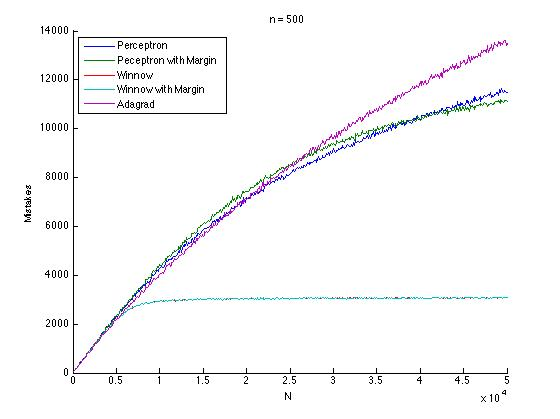
\includegraphics[scale=0.5]{HW3_code/n500}\\
  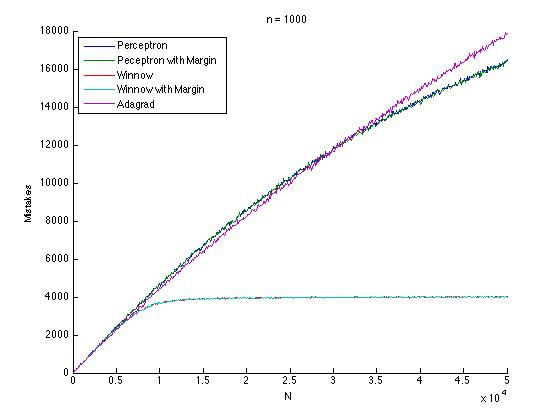
\includegraphics[scale=0.5]{HW3_code/n1000}\\
You might not be able to see, but Winnow and Winnow with Margin have very similar number of mistakes for a given input size, and are overlapping one another on the graph. Both flatten off in mistakes fairly quickly. In general, Adagrad grows linearly with input size, and very slowly begins to flatten off after a huge input size, while Perceptron and Perceptron with Margin begin to flatten off sooner. With n=1000 vs. n=500, the notable difference is that it takes longer (as in starting at a larger N) for each algorithm to begin flattening off. This makes sense since n=1000 is a much higher dimensional space than n=500, and so it takes more data to ``narrow'' down the space.\\\\
About an hour before the assignment deadline, I realized I was calculating the plot in a sort of $n^2$ operation, where I generate a new dataset for each N, and iterate up to that point counting the mistakes, then reset, create a new dataset for N+1, count up, etc... So I quickly wrote the ``memoized'' version as was probabily intended, where the dataset of 50,000 is generated once, and the mistakes are counted up to the 50,000, while preserving the past number of mistakes. This took about a minute to evaluate, and is the code I've included in the *\_error.m files. The graphs are:
 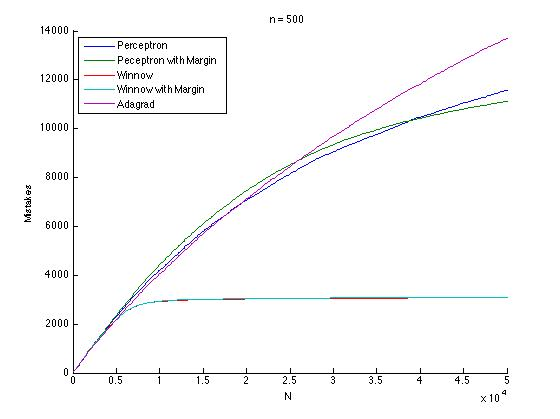
\includegraphics[scale=0.5]{HW3_code/n500_memoize}\\
 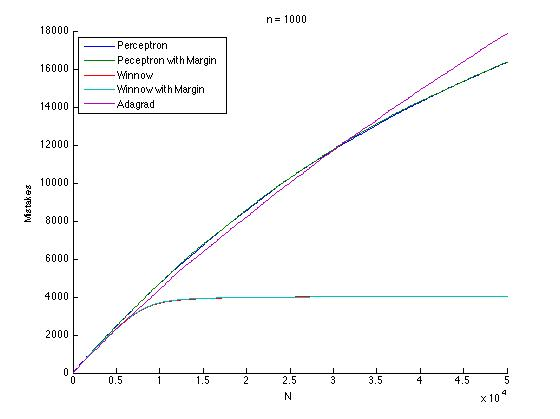
\includegraphics[scale=0.5]{HW3_code/n1000_memoize}\\
As expected, there's not so much noise (or jiggling around) in the graph this time around, since the same dataset is used. However, the overall trends and magnitutdes of the plots are about the same, since the ``sample size'' of the randomly generated datasets are so large.







\item Learning Curves of Online Learning Algorithms\\\\
I did the exact same thing to get the optimal parameters, as I did in the first problem. The script is in getParameters2.m\\
I iterated on my classifiers to make them repeat until the string of R=1000 successful classifications. I put these functions in perceptron\_R.m, perceptron\_margin\_R.m, winnow\_R.m, winnow\_margin\_R.m, and adagrad\_R.m.\\
    \begin{table}[H]
    \begin{tabular}{|p{4.7cm}<{\centering}|p{2.0cm}<{\centering}|p{1.5cm}<{\centering}|p{1.5cm}<{\centering}|p{1.5cm}<{\centering}|p{1.5cm}<{\centering}|p{1.5cm}<{\centering}|}
      \hline
      \multirow{2}{*}{Algorithm} & \multirow{2}{*}{Parameters} & \multicolumn{5}{|c|}{Data Set} \\
      \cline{3-7}
 & & $n=40$& $n=80$& $n=120$& $n=160$& $n=200$\\
 \hline
     % Perceptron    & $\eta$               &                             &   & & &                              \\\hline \hline
      Perceptron w/margin &          $\eta$          &1.5                   &1.5     &0.03 &0.03 &0.03                              \\\hline

      %& $\gamma$ &  & & & &\\ \hline \hline
      Winnow               &     $\alpha$           &1.1                     &1.1         &1.1 &1.1 &1.1                          \\\hline %\hline
      \multirow{2}{*}{Winnow w/margin}     & $\alpha$&1.1                                     &1.1     &1.1 &1.1 &1.1                \\
      \cline{2-7}
      & $\gamma$ &2.0  &2.0 &2.0 &2.0 &2.0\\ \hline %\hline
      AdaGrad             & $\eta$&1.5                                      &1.5               &1.5 &1.5 &1.5                    \\\hline %\hline
      %\multirow{2}{*}{AdaGrad w/margin}    & $\eta$&                                               &   & & &                                \\
%      \cline{2-7}
%      & $\gamma$ &  & & & &\\ \hline
    \end{tabular}
    \end{table}

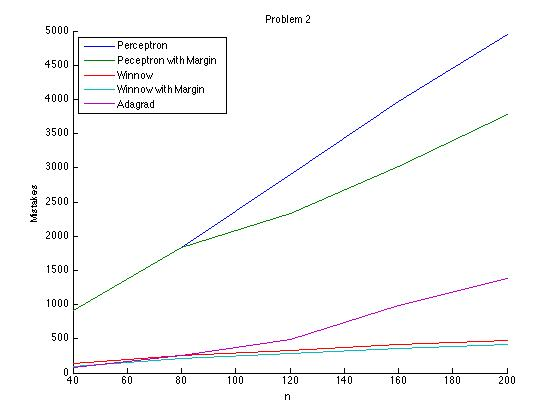
\includegraphics[scale=0.5]{HW3_code/problem2}\\
The above graph was generated with numErrors2.m. As I kind of alluded to in the last problem, the number of mistakes to reach a relatively reliable state (just defined by having no mistakes 1000 in a row...) increases with n. Winnow, Winnow with Margin, and Adagrad ``converged'' in this sense, relatively quickly, while Perceptron and Perceptron with Margin made many more mistakes.\\
Also, it's interesting to note that Adagrad seems to be growing in mistakes faster than linearly with n, although it's hard to say if that's true because of the very very small sample size (only 5 points on a graph).







\item Use Online Learning Algorithms As Batch Learning Algorithms\\\\
Again, I obtained the parameters similarly as to how I did in problems 1 and 2. The code for this is in getParameters3.m.\\\\
      \begin{center}
  \begin{table}[H]
    \begin{tabular}{|p{4.3cm}<{\centering}|p{2.5cm}<{\centering}|p{2.7cm}<{\centering}|p{2.7cm}<{\centering}|p{2.7cm}<{\centering}|}
      \hline
      \multirow{2}{*}{Algorithm} & \multirow{2}{*}{Parm \& Accy} & \multicolumn{3}{|c|}{Data Set} \\
      \cline{3-5}
 & & $m=100$& $m=500$& $m=1000$\\
 \hline
      Perceptron    & Accy \%               &0.978                             &0.801   &0.808                               \\ \hline
%      \cline{2-5}
%      & Accy\% &0.967  &0.988 &0.992 \\ \hline \hline
      \multirow{2}{*}{Perceptron w/margin} &          $\eta$          &1.5                   &0.25     &0.25                              \\
      \cline{2-5}
      %& $\gamma$ &  & & \\
      %\cline{2-5}
      & Accy\% &0.978  &0.905 &0.809 \\ \hline \hline
      \multirow{2}{*}{Winnow}               &     $\alpha$           &1.1                     &1.1         &1.1                           \\
      \cline{2-5}
      & Accy\% &0.939  &0.828 & 0.779\\ \hline \hline
      \multirow{3}{*}{Winnow w/margin}     & $\alpha$&1.1                                     &1.1     &1.1                \\
      \cline{2-5}
      & $\gamma$ &0.3  &2.0 & 0.04\\
      \cline{2-5}
            & Accy\% &0.944  &0.822 & 0.796\\ \hline \hline
      \multirow{2}{*}{AdaGrad}             & $\eta$&1.5                                      &1.5               &1.5                     \\
      \cline{2-5}
      & Accy\% &0.930  &0.759 & 0.816\\ \hline %\hline
      %\multirow{3}{*}{AdaGrad w/margin}    & $\eta$&                                               &   &                                \\
%      \cline{2-5}
%      & $\gamma$ &  & &\\
%      \cline{2-5}
%      & Accy\% &  & & \\\hline
    \end{tabular}
    \end{table}
    \end{center}

The numbers were generated with number3.m. In general, we see that as m increases, the accuracy decreases. The table holds the optimal parameters and the accuracies from part d.\\\\
The accuracies in order from greatest to least accuracies are : Perceptron with Margin, Perceptron, Winnow with Margin, Winnow, and then Adagrad. This is in contrast with the ``winners'' of problem 2, where Perceptron and Perceptron with Margin were making a huge number of mistakes (relative to the others) to reach that ``stable'' state. This suggests that the two Perceptron algorithms should be trusted more when used as batch algorithms. Since they were making so many mistakes for so long, if the training data was small, the Perceptrons would perform pretty poorly. 





\item Bonus\\\\
 Since there are much less positive examples than negative examples, whenever we see a positive example, it's much more of an event, and so we need to update accordingly. To do this, I just took my old Perceptron with Margin, and made two separate margins, one for positive examples, and one for negative. The positive margin has to be much larger than the negative one since we want it to have a bigger ``impact.'' I toyed around with my margins, and $\gamma_+ = 1$, and $\gamma_- = 0$ seemed to work well. Over 10 trials, the average results were as follows:\\
      \begin{center}
  \begin{table}[H]
    \begin{tabular}{|p{4.3cm}<{\centering}|p{2.5cm}<{\centering}|p{2.7cm}<{\centering}|p{2.7cm}<{\centering}|p{2.7cm}<{\centering}|}
      \hline
      \multirow{2}{*}{Algorithm} & \multirow{2}{*}{Accy} & \multicolumn{3}{|c|}{Data Set} \\
      \cline{3-5}
 & & $m=100$& $m=500$& $m=1000$\\
 \hline
      Perceptron    & Accy \%               &0.9901                             &0.9489   &1.0                              \\ \hline
%      \cline{2-5}
%      & Accy\% &0.967  &0.988 &0.992 \\ \hline \hline
      Bonus Perceptron & \\
      & Accy\% &0.978  &0.905 &1.0 \\ \hline \hline
    \end{tabular}
    \end{table}
    \end{center}
So this new updated algorithm outperforms, or ties with the old perceptron. The code to compare the two is in bonus.m, and my new perceptron is in perceptron\_bonus.m.
\end{enumerate}

\end{document}

